\documentclass[../AISTR.tex]{subfiles}
\begin{document}

\section{Создание сервера обмена сообщениями по протоколу TCP}
\subsection{Принцип работы в сетях TCP/IP}
\textbf{TCP/IP} — сетевая модель передачи данных, представленных в цифровом виде. Протокол \tcp -- протокол транспортного уровня согласно модели \osi (см. \refris{fig:osi}).

Основное достоинство протокола -- ориентированность на ``качество'' соединения. \tcp устанавливает предварительное соединение, а затем проверяет, действительно ли файл дошёл до получателя \cite{kumar_survey_2012}. 

На \refris{fig:handshake} показано, как устанавливается соединения между устройствами по протоколу \tcp (технология тройного рукопожатия):
\begin{figure}[h]
	\centering
	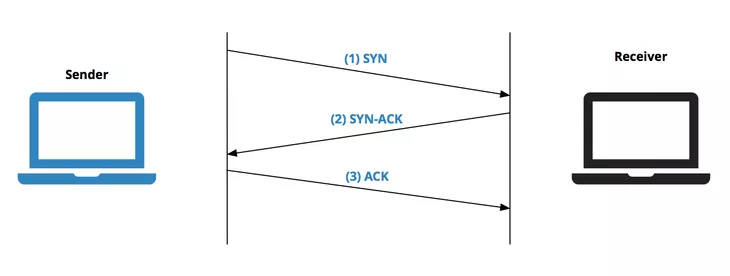
\includegraphics[width=0.8\linewidth]{../images/handshake}
	\caption{Установка соединения протоколом \tcp}
	\label{fig:handshake}
\end{figure}
\begin{enumerate}
	\item Клиент отсылает серверу пакет с флагом SYN. Этот начальный пакет позволяет клиенту установить, каким должен быть первый порядковый номер для пакетов запроса;
	\item Сервер, получив пакет, добавляет к нему флаг ACK и отсылает клиенту. Этот пакет подтверждает порядковый номер, отправленный клиентом, подтверждая его. Однако сервер также должен отправить SYN и порядковый номер обратно клиенту, чтобы установить, каким должен быть первый порядковый номер для пакетов ответа, исходящих от сервера;
	\item Наконец, клиент отвечает на пакет SYN / ACK пакетом ACK, который подтверждает запрос порядкового номера сервера.
\end{enumerate}



\subsection{Принцип работы программы}
Программа состоит из двух частей:
\begin{enumerate}
	\item Клиент;
	\item Сервер;
\end{enumerate}
Программа работает следующим образом (см. \refris{fig:tcp-server}): 

\begin{figure}[p]
	\centering
	\includegraphics[trim=70 555 195 80,clip,width=0.8\linewidth]{"../images/схема tcp"}
	\caption{Схема работы серверной части}
	\label{fig:tcp-server}
\end{figure}

\begin{enumerate}
	\item Производится запуск сервера;
	\item Производится запуск клиента;
	\item С клиента поступает запрос на подключение, который всегда одобряется;
	\item После подключения сервер отправляет клиенту сообщение об успешном подключении (этого можно было не делать, поскольку успешность подключения обеспечивается протоколом \tcp).
\end{enumerate}

После этого клиент может передать серверу файл. Контроль за передачей файла ведётся из консоли сервера, а также в графическом интерфейсе клиента.

\subsection{Реализация кода программы}
\begin{enumerate}
	\item \textbf{Запуск сервера.} На листинге \rbf{list:server_init} приведён метод, осуществляющий запуск сервера на порт $9999$.
	\begin{lstlisting}[caption=Метод запуска сервера,captionpos=b, label={list:server_init}]
		void myserver::startServer()
		{
			if (this->listen(QHostAddress::Any,9999))
			{
				qDebug()<<"Listening";
			}
			else
			{
				qDebug()<<"Not listening";
			}
		}
	\end{lstlisting}
	\item При \textbf{поступлении входящего запроса} реализуется метод, приведённый в листинге \rbf{list:server_connect}:
	\begin{lstlisting}[caption=Метод входящего подключения,captionpos=b, label={list:server_connect}]
		void myserver::incomingConnection(qintptr socketDescriptor)
		{
			socket = new QTcpSocket(this);
			socket->setSocketDescriptor(socketDescriptor);
			connect(socket,SIGNAL(readyRead()),this,SLOT(sockReady()));
			connect(socket,SIGNAL(disconnected()),this,SLOT(sockDisc()));
			qDebug()<<socketDescriptor<<" Client connected";			
			socket->write("You are connect");
			qDebug()<<"Send client connect status - YES";
		}
	\end{lstlisting}
\end{enumerate}
\subsection{Терминал сервера}
Сервер не нуждается в графической оболочке, ему достаточно выводить текст в консоль посредством встроенных в Qt средств (qDebug()). На \refris{fig:serverstart} показан вывод при запуске сервера.

На \refris{fig:serverconnected} показан вывод сообщения при подключении клиента к сервера. $5$ -- уникальный номер соединения. 

На последнем \refris{fig:serverreceived} выведено сообщение при получении сервером файла. 
 
\begin{figure}[p]
	\centering
	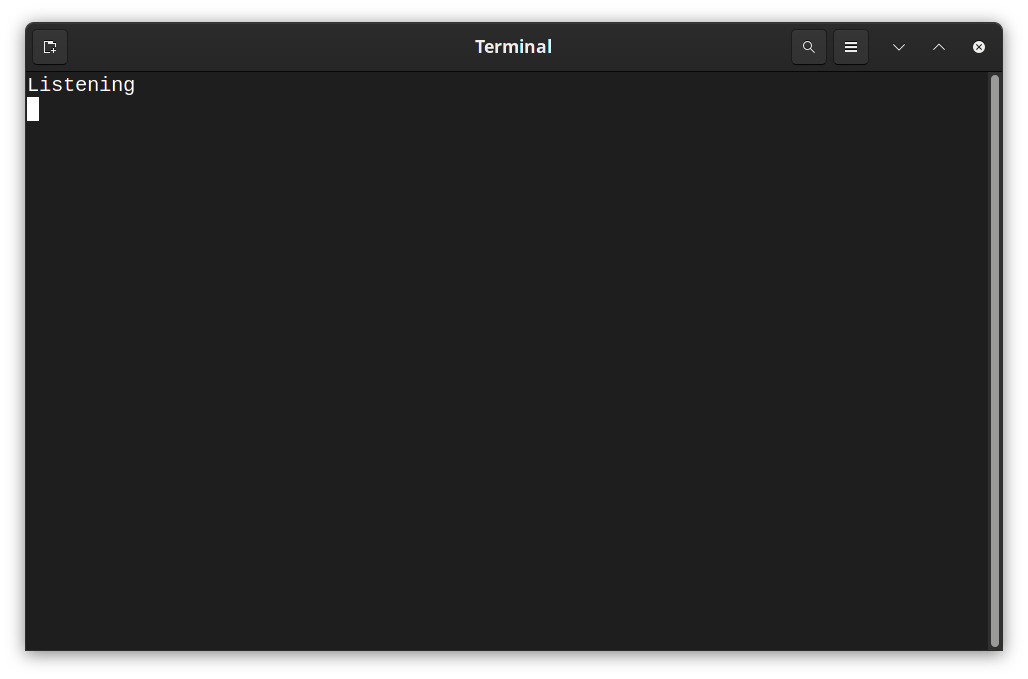
\includegraphics[width=\linewidth]{../images/server_start}
	\caption{Запуск сервера}
	\label{fig:serverstart}
\end{figure}


\begin{figure}[p]
	\centering
	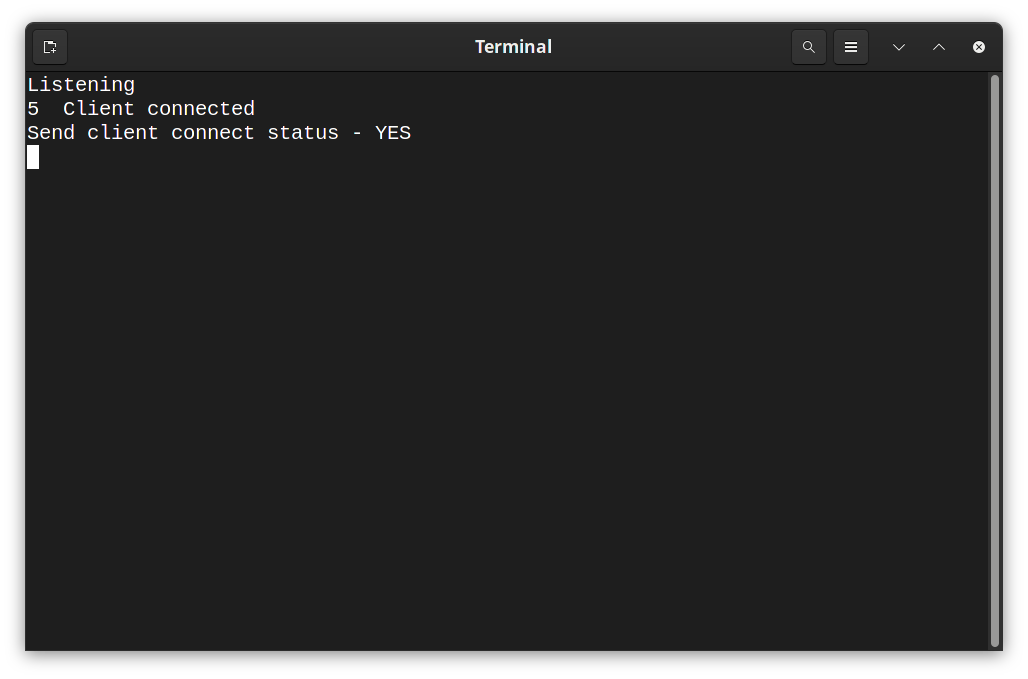
\includegraphics[width=\linewidth]{../images/server_connected}
	\caption{Подключение клиента к серверу}
	\label{fig:serverconnected}
\end{figure}

\begin{figure}[p]
	\centering
	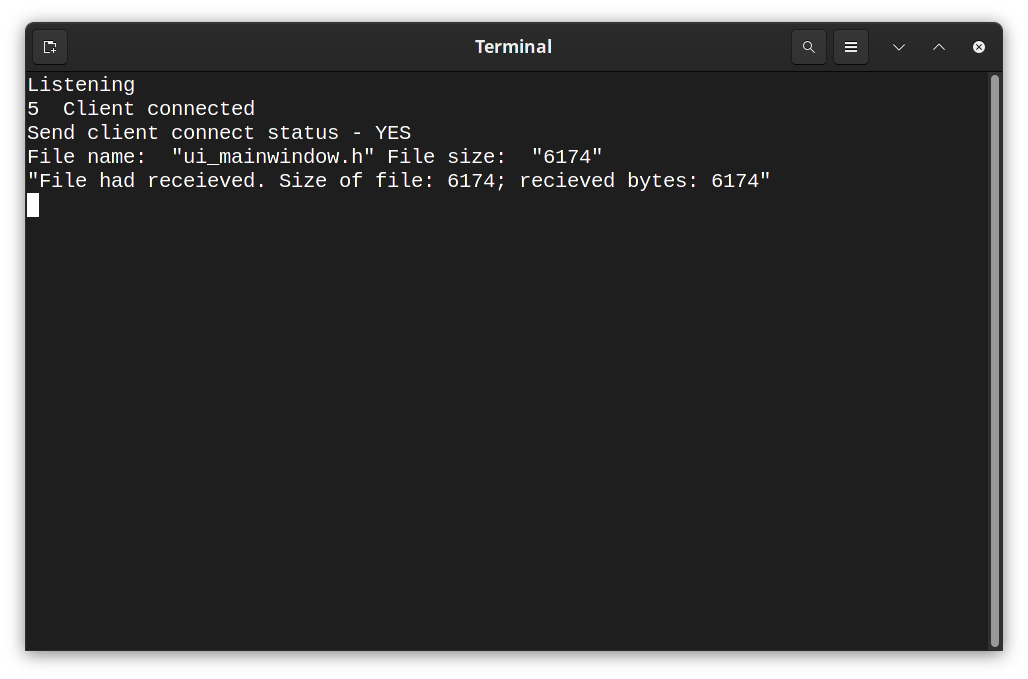
\includegraphics[width=\linewidth]{../images/server_received}
	\caption{Получение файла от сервера}
	\label{fig:serverreceived}
\end{figure}
\end{document}